As discussed above, one can induce periodic undamped oscillations within TSAs by conserving mechanical energy of the system. This can be achieved by a proper selection of control algorithm, and this approach is commonly known in literature as energy preserving control (EPC). The following provides a brief introduction into the EPC and discusses design and implementation of this control strategy to twisted string actuators.

The concept of energy-preserving control has been originally proposed by Wiklund et al. who demonstrated an approach to solve the swing-up problem of inverted pendulum with this control strategy \cite{wiklund1993new}. The EPC technique was later applied to other underactuated systems (Furuta pendulum, acrobot, three-link gymnast robot, cart-pole) in the works of Iwashiro and Spong, with the studies outlining regulation methods to reach desired energy levels even in the presence of actuator constraints \cite{iwashiro1996energy,spong1996energy}.
Fantoni et al. have later demonstrated how, using the passivity properties of the internal energy of a pendubot system, one can bring the state either arbitrarily close to the top position or to some homoclinic orbit  \cite{fantoni2000energy}. %Research into energy-based control for the underactuated systems is still going on. % This is how real-time energy control of the cart-pole was presented in the article \cite{kennedy2019real}. This controller used a novel barrier function to make the swing-up method. This feature allows using the energy-based controller for real-time implementation.
%The sequence of papers by Maalouf and colleagues  \cite{maalouf2017energy,maalouf2020biomimetic} demonstrated the compatibility of energy-based control for humanoid robots in push recovery during quiet standing scenario. Case-study demonstrated that energy-based control is more efficient in terms of cumulative work than PID control and controlled Lagrangian approach. Additionally to energy efficiency, authors highlighted that energy-based control performance required in some setups the same (inverted pendulum on a cart) or up to 3 times lower-order (inverted pendulum) of peak control torque on actuator comparing with PID and controlled Lagrangian. This property of energy-based control could be used in low-power motor systems.
In addition, the EPC was successfully applied in robot control tasks. For instance, Asano et al. have used this technique to control a bipedal walking robot and discovered that the application of energy constraints has significantly simplified generation of movement patterns \cite{asano2004novel}.

\subsection{Fundamentals of Energy-Preserving Control}

One of the most powerful features of the energy preserving control method is that it becomes much simpler to design a regulator for a particular dynamical system. One starts the EPC design process by driving a single energy equation of the system $E(q)$, where $q$ is a scalar position. In order to reach some desired position $q_d$, one therefore needs to reach constant desired energy level $E_d = E(q_d)$. Then, defining the energy error with
\begin{equation*}
    \tilde{E} = E_d - E(q)
\end{equation*}
and choosing control law as
\begin{equation}\label{eq.con:epc}
    u = k\tilde{E}\dot{q}
\end{equation}
results in energy error converging to zero, which will eventually drive system energy to desired level $E_d$. This may be shown by analyzing the Lyapunov candidate 
\begin{equation}\label{eq:v_dot}
    V = \frac{1}{2}\tilde{E}^2
\end{equation}
whose derivative can be found as follows:
\begin{equation}\label{eq:v_dot}
    \dot{V} = \tilde{E}\dot{\tilde{E}} = \tilde{E} ( \dot{E}_d - \dot{q} u) = -\tilde{E} \dot{q}^T u= -k\tilde{E}^2\dot{q}^2
\end{equation}
which is strictly negative along all system trajectories, provided that $\dot{q}\neq0$. For more details on stability analysis of this control scheme the reader is kindly referred to the works \cite{iwashiro1996energy,spong1996energy}.

Now, let us move onto implementation of energy preserving control in the linear TSA joint studied in the previous section.
 
\subsection{Experiment with a Linear TSA}

We have conducted an experiment whose main goal was to induce TSAs load oscillation with amplitude of $X_d = 20$ mm starting from a fully untwisted configuration. the mass was setted to be $\hat{m} = 2$ kg which corresponds to the energy level of $E = 0.39$ J. In addition, maximal motor torque was set to be 6 mNm. 

In order to regulate to the desired energy level we have implemented control law \eqref{eq.con:epc}, with actual energy provided by equation \eqref{eq.mod:total_energy} except for the dissipative term $E_D$: 
\begin{equation}\label{eq.con:total_energy}
    E = \frac{1}{2} \hat{I}\dot{\theta}^2 + \frac{1}{2}\hat{m} \dot{X}^2 + \hat{m}gX
\end{equation}
where $\hat{I}, \hat{m}$ denote our estimates of the motor inertia and payload mass, respectively. The value of motor inertia was identified to be $\hat{I}=9.7$ gcm$^2$. 
Load position $X$ was measured directly while $\dot{\theta},\dot{X}$ was estimated with backward difference with data sampling frequency of 3 kHz. No other computations or measurements were necessary for energy calculations.

Time plots of resulting payload motion and motor torque are presented in Figure \ref{fig:time_plots_X_torque_epc}. One can note that it takes the controller about 2.5 periods in as many seconds to reach desired contraction levels, while the motor torque remains bounded. Motor controller had a hardware cutoff at 6 mNm torque, which is shown by a horizontal dashed line in  Fig. \ref{fig:time_plots_X_torque_epc} (bottom), while the intermittent peaks exceeding these values are the result of noise in electrical current measurements that were used to compute motor torque.
For the sake of comparison, if one simply commands the motor to twist the strings and drive the payload to the desired contraction level with the same torque constraint of 6 mNm, the load gets after travelling approximately 3 mm, as shown by the curve labeled `PD control' in Fig. \ref{fig:time_plots_X_torque_epc} (top). 

\begin{figure}
		\centering
		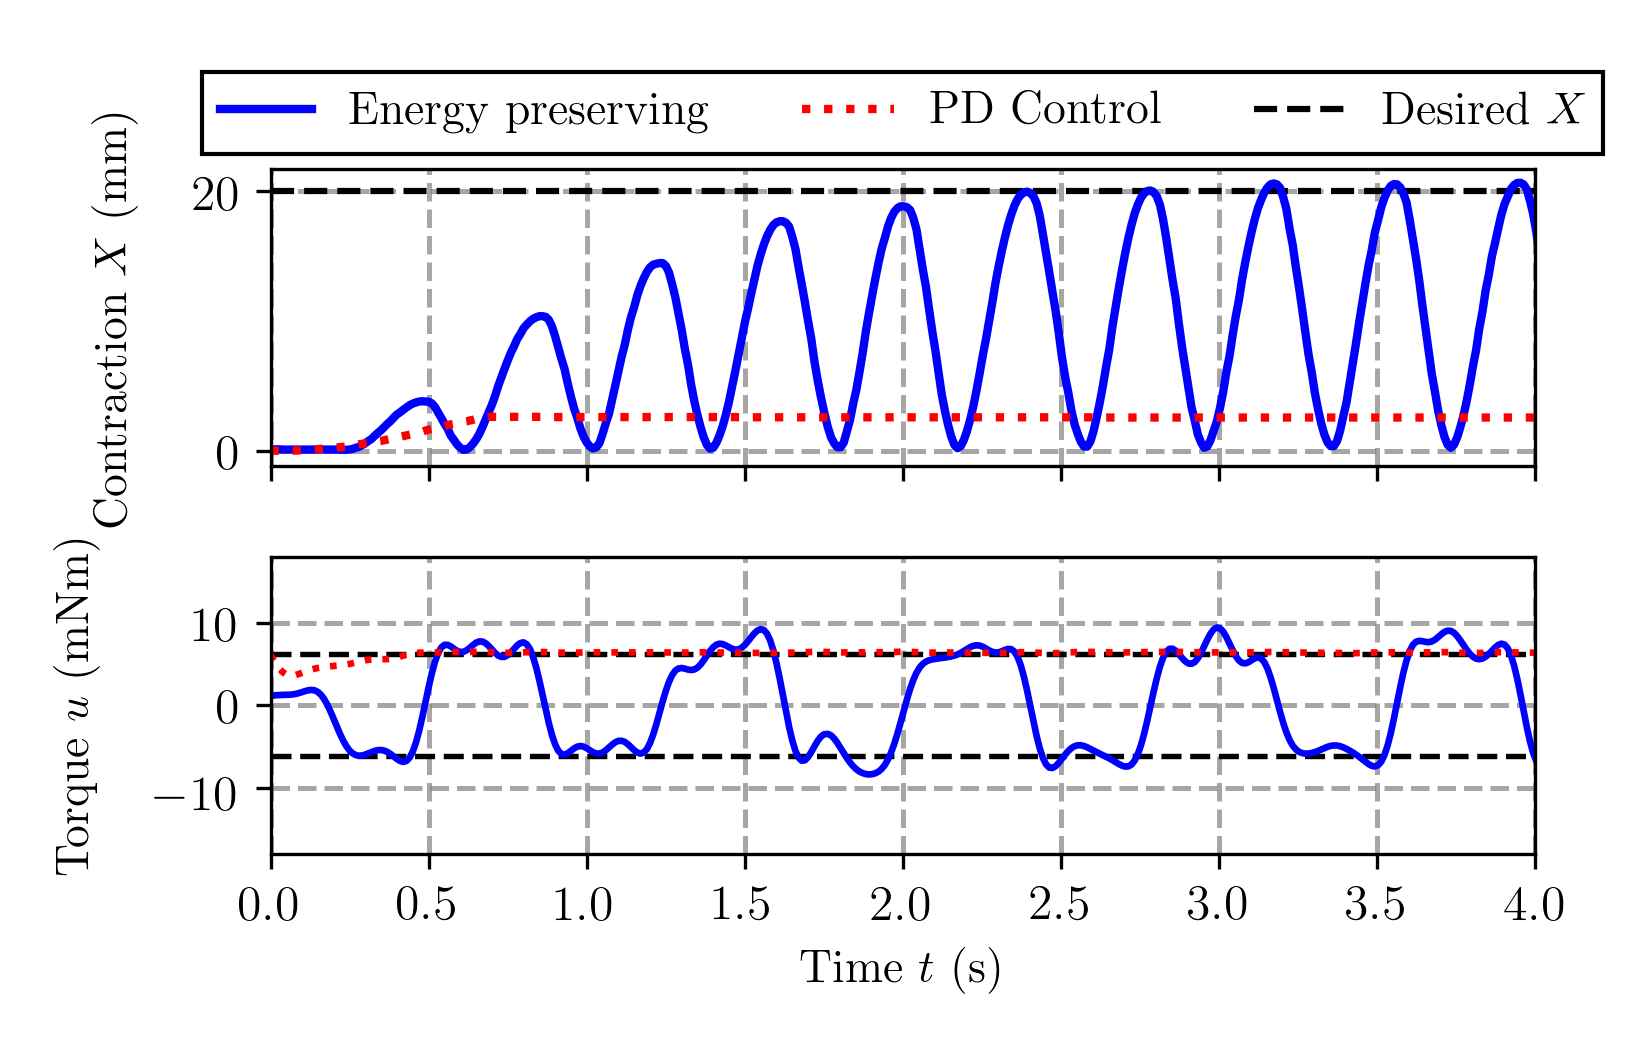
\includegraphics[trim= 0.0cm 0.8cm 0.0cm 0.0cm,width=1.0\columnwidth]{pics/plots/control_comparison.png}
		\caption{Experimental time plots of payload position (top) and motor torque (bottom) in a TSA with energy-preserving control and torque constraints}
 		\label{fig:time_plots_X_torque_epc}
		\vspace*{-2mm} 
\end{figure}

Once the desired energy level has been reached, the controller conserves it throughout the experiment, as shown in Fig. \ref{fig:energy_levels_EPC}. The corresponding phase plots in the actuator and payload space are shown in Fig. \ref{fig:phase_plot_EPC}. One can note with the help of overlaid vector fields (computed with the proposed mathematical model) that oscillations starting from the origin diverge toward the final limit cycle, while those that start outside converge to it, which suggests stable controller behavior. The same observation holds for both motor and payload responses.
\begin{figure}
		\centering
		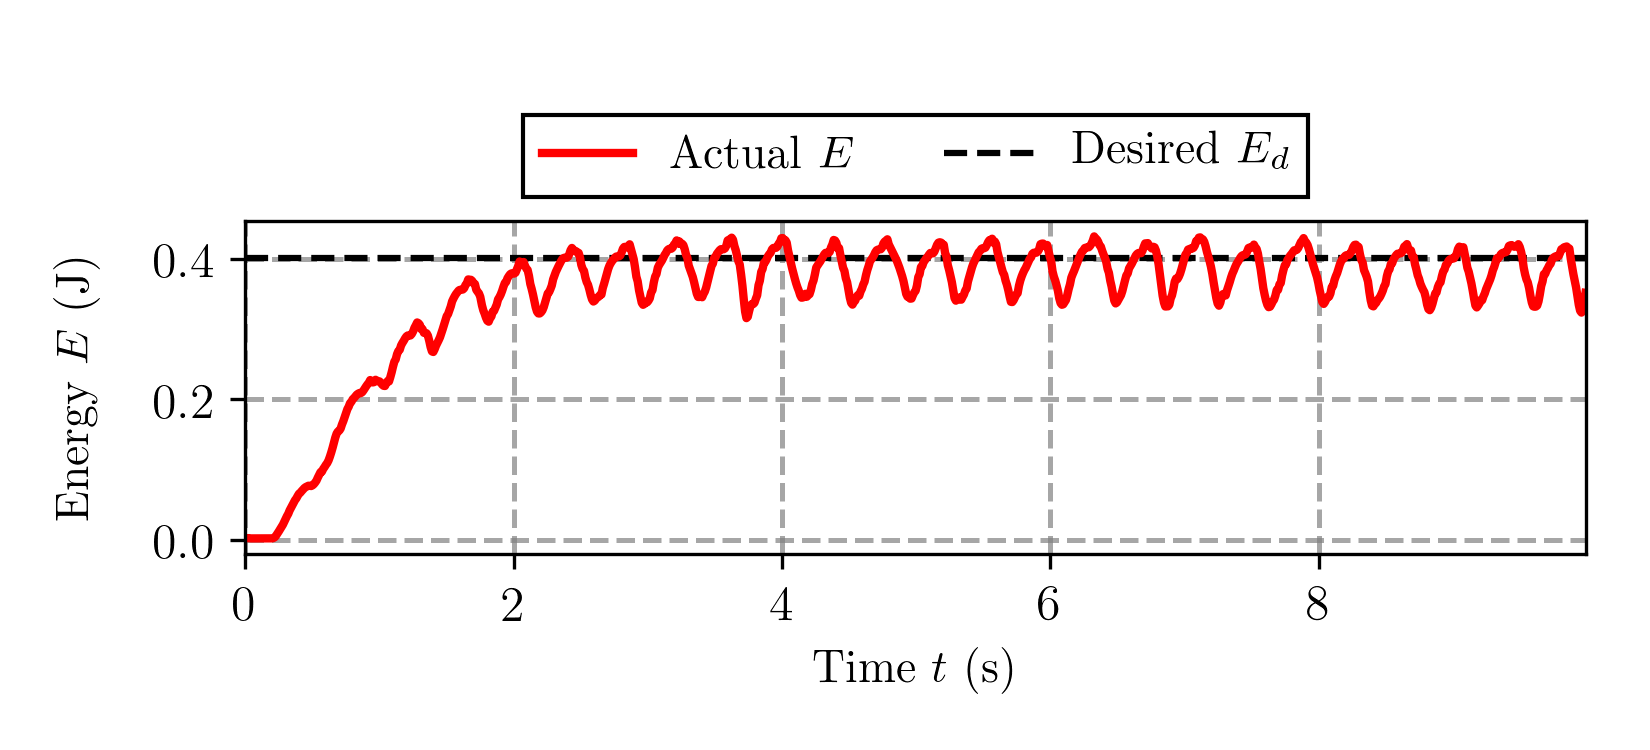
\includegraphics[trim= 0.0cm 1.0cm 0.0cm 0.0cm,width=1.0\columnwidth]{pics/plots/energy_convergence.png}
		\caption{Desired and actual energy levels in TSA under energy preserving control}
 		\label{fig:energy_levels_EPC}
		\vspace*{-2mm} 
\end{figure}

\begin{figure}
		\centering
		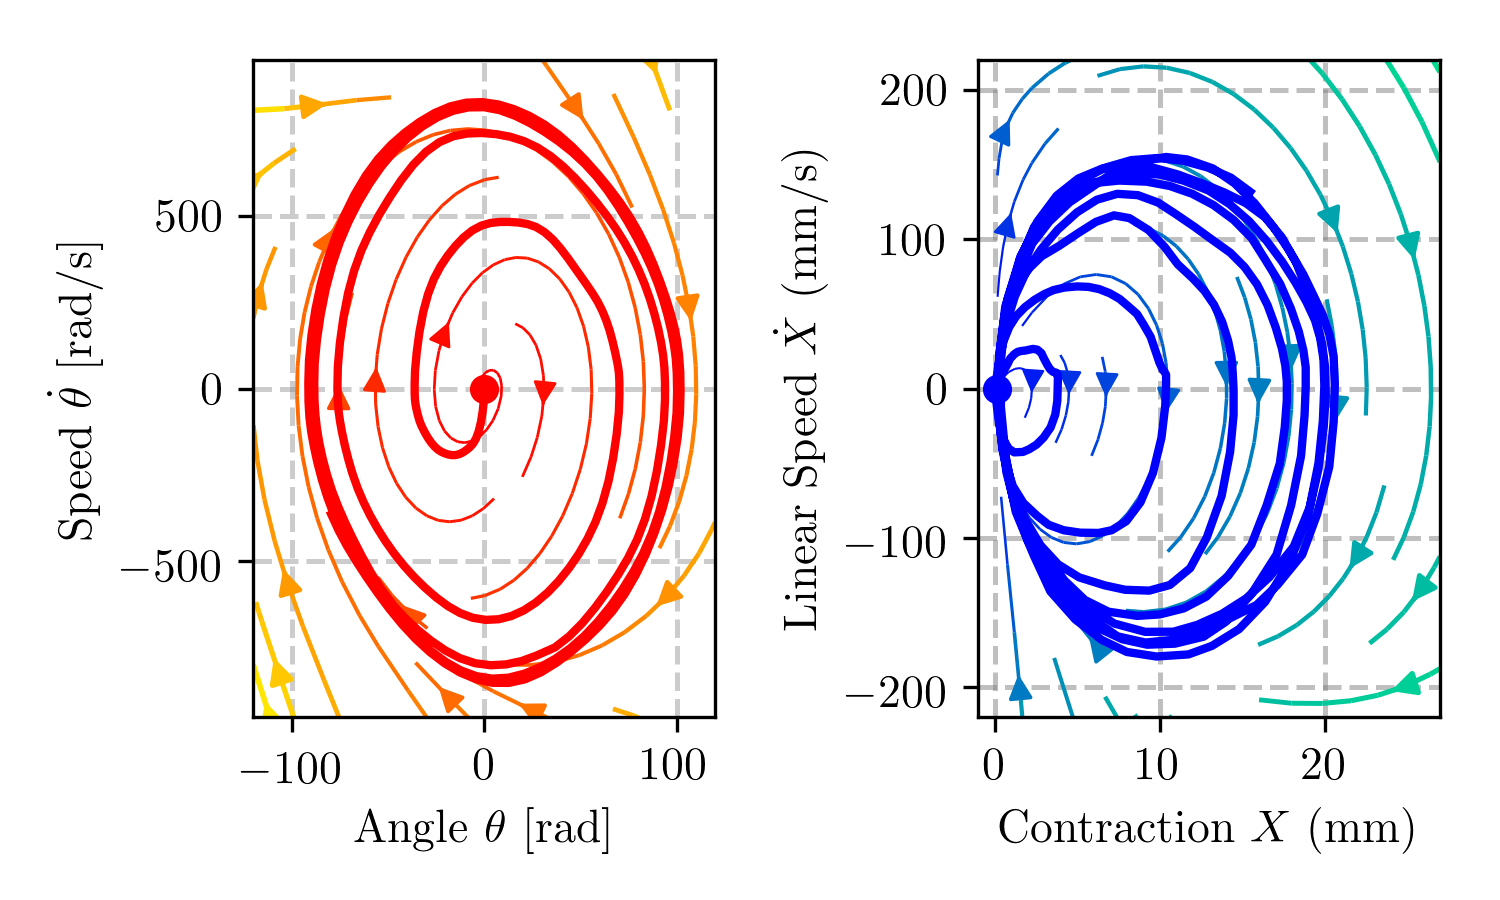
\includegraphics[trim= 0.0cm 0.8cm 0.0cm 0.0cm,width=1.0\columnwidth]{pics/plots/phase_space_control.png}
		\caption{Phase portraits of TSA in actuator (left) and payload (right) space with energy preserving control. Vector fields are generated with proposed mathematical model}
 		\label{fig:phase_plot_EPC}
		\vspace*{-2mm} 
\end{figure}

These experiments confirm that energy preserving control can indeed be successfully implemented in twisted string actuators to generate undamped oscillatory response with nearly-constant energy levels, as was suggested by our initial hypothesis. Design of controllers of this type is fairly simple and straightforward, and therefore these results seem very encouraging. 

